\documentclass[../report.tex]{subfiles}
\begin{document}

\section {数据库设计}

\subsection {数据库设计需求}

学校有多个校区,各个校区均有其校区代码(唯一)、校区名称和校区地址
(实体中包括但不限于上述属性,下同)。学校开设多个专业,各个专业均有其
专业代码(唯一)、专业名称、专业地址、专业负责人和所属校区(一个专业仅
属于一个校区)。学校建立多个班级,各个班级均有其班级代码(唯一)、班级
名称、建班年月、班主任、所属年级(年份)和所属专业。

学校将所有教师和学生的基本个人信息统一存放,包括身份证件号(唯一)、
身份证件类型(身份证或护照)、中文名称、性别码(女或男)、出生日期(年
月日)和国籍(中文名称)。如果教师和学生提供了家庭通讯方式,包括家庭住
址、家庭邮政编码和家庭电话,学校也会记录。每个教师也有属于自己的工号(唯
一),每个学生有属于自己的学号(唯一)。学校记录学生的入学年月、电子邮
箱和所属班级,也记录教师的入职年月、电子邮箱、所属专业和职称(教授或副
教授)。学校允许学生转专业和降级(二者不同时发生,转专业和降级时均转班,
且只允许一次转专业和一次降级),统称为学籍异动。学生发生学籍异动时需要
记录异动编号(唯一,同一学生转专业和降级各有不同的异动编号)、异动日期
(年月)、原班级代码和现班级代码。转专业还需要记录是否已转出团员关系(是、
否或不是团员),降级则还需要记录降级原因(休学或支教)。

学校开设不同课程,每门课程均有其课程号(唯一,与课程名称一一对应)、
课程名称、开课专业和考核方式(考试或当堂答辩,满分均为 100)。当一门课
程开课时,需要记录其授课教师(一门课仅有一个授课教师)、开课日期(年)、
开课学期(春或秋)、开课时间(每个课程一周只开一节课,为周一至周五的第
一节至第九节中的某一节,自定义记录方式)。学校会记录每个学生的选课记录
(不允许重复选课),包括选课日期(同开课日期)、选课学期(同开课学期)
和考试成绩。

\subsection {数据库设计}

这里结合第二次实验的设计报告,去给出我们最后选择的数据库设计。

\begin{figure}
\centering
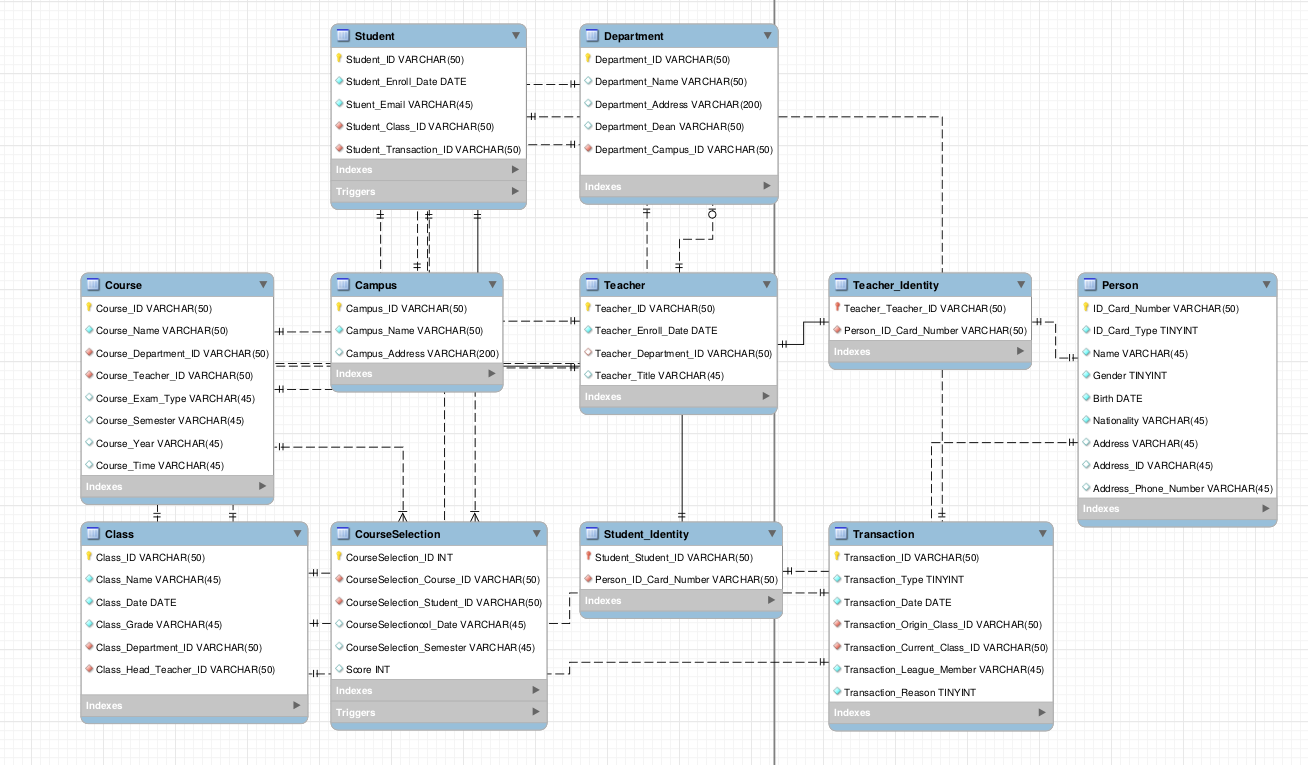
\includegraphics[width=1\linewidth]{../figure/database-design.png}
\caption{数据库设计一览}
\label{fig:database-design}
\end{figure}


\end{document}